\documentclass[border=8pt]{standalone}
\usepackage{tikz}
\usetikzlibrary{arrows.meta,positioning,calc,fit}
\begin{document}
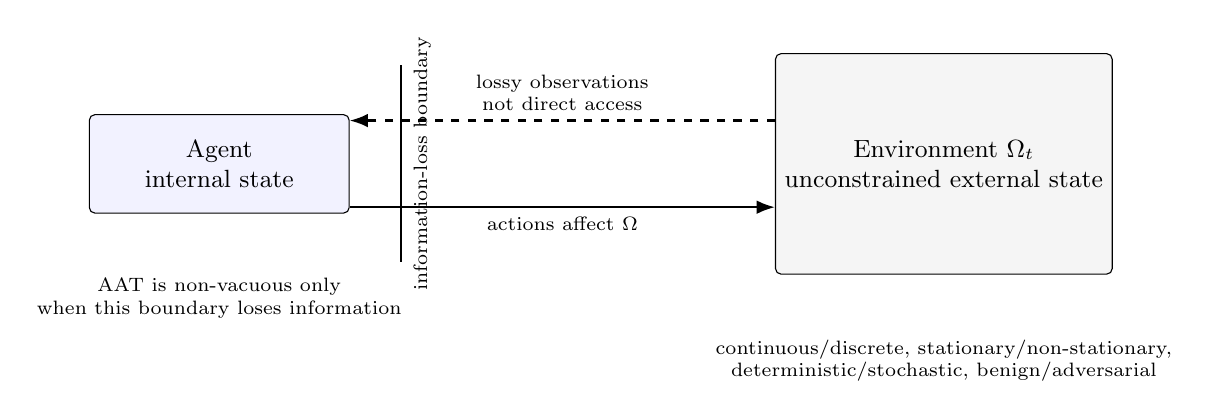
\begin{tikzpicture}[
  box/.style={draw, rounded corners=2pt, align=center, minimum width=3.3cm, minimum height=1.25cm, font=\small},
  channel/.style={-Latex, thick},
  lossy/.style={-Latex, thick, dashed},
  note/.style={align=center, font=\scriptsize}
]

\node[box, fill=blue!5] (agent) {Agent\\internal state};
\node[box, fill=gray!8, right=5.4cm of agent, minimum width=4.0cm, minimum height=2.8cm] (env) {Environment $\Omega_t$\\unconstrained external state};

\coordinate (obsA) at ($(env.west)+(0,0.55)$);
\coordinate (obsB) at ($(agent.east)+(0,0.55)$);
\coordinate (actA) at ($(agent.east)+(0,-0.55)$);
\coordinate (actB) at ($(env.west)+(0,-0.55)$);

\draw[lossy] (obsA) -- node[above, note] {lossy observations\\not direct access} (obsB);
\draw[channel] (actA) -- node[below, note] {actions affect $\Omega$} (actB);

\draw[thick] ($(agent.east)+(0.65,1.25)$) -- ($(agent.east)+(0.65,-1.25)$);
\node[note, rotate=90] at ($(agent.east)+(0.92,0)$) {information-loss boundary};

\node[note, below=0.7cm of agent] {AAT is non-vacuous only\\when this boundary loses information};
\node[note, below=0.7cm of env] {continuous/discrete, stationary/non-stationary,\\deterministic/stochastic, benign/adversarial};

\end{tikzpicture}
\end{document}
